\chapter{Methods}
%\section{Sample preparation}
%The thorium doped PbS thin film was prepared by chemical bath deposition (CBD) before the present work began. Templeman et al. 2017 \cite{Templeman2017} describe the process in detail, but it is summarized here for completion. The GaAs (100) substrate was submerged in a chemical bath containing thorium 228. The thorium concentration, temperature, and pH were all precisely varied to control the concentration of thorium incorporated into the PbS rock salt lattice; a method that was confirmed to work by Biton et al. 2014 \cite{Biton2014}. The thorium added to the solution had already aged $\sim$2.5 years since it was created in presumably pure form. Therefore, its daughters were also present in the solution, and Templeman et al. confirmed by gamma and alpha spectroscopy that at least some of the daughters were incorporated into the lattice as well, though they did not attempt to deduce or measure concentrations. The sample properties as reported by Templeman et al. 2017 are collected in Table \ref{sample_properties} and a photo of the sample can be seen in Figure \ref{photo_of_thin_film_sample}.
%
%%\begin{table}[hb]
%%\begin{center}
%%\begin{tabular}{|l|l|}\hline
%%Substrate						&	GaAs (100) \\\hline
%%Dimensions					&	1 cm x 1.5 cm \\\hline
%%Film thickness					&	$\sim$500 nm \\\hline
%%Grain size						&	$\sim$150 nm \\\hline
%%Th 228 concentration			&	0.15 ppm \\\hline
%%Total activity*					&	65 Bq \\\hline
%%Sample creation date			&	22 Jul 2016\\\hline
%%\end{tabular}
%%\end{center}
%%\label{sample_properties}
%%\caption{Sample properties reported by Templeman et al. 2017 \cite{Templeman2017}. * Total activity measured a brief but unknown time after sample preparation.}
%%\end{table}
%
%
%\begin{figure}
%\begin{floatrow}
%\ffigbox{%
%  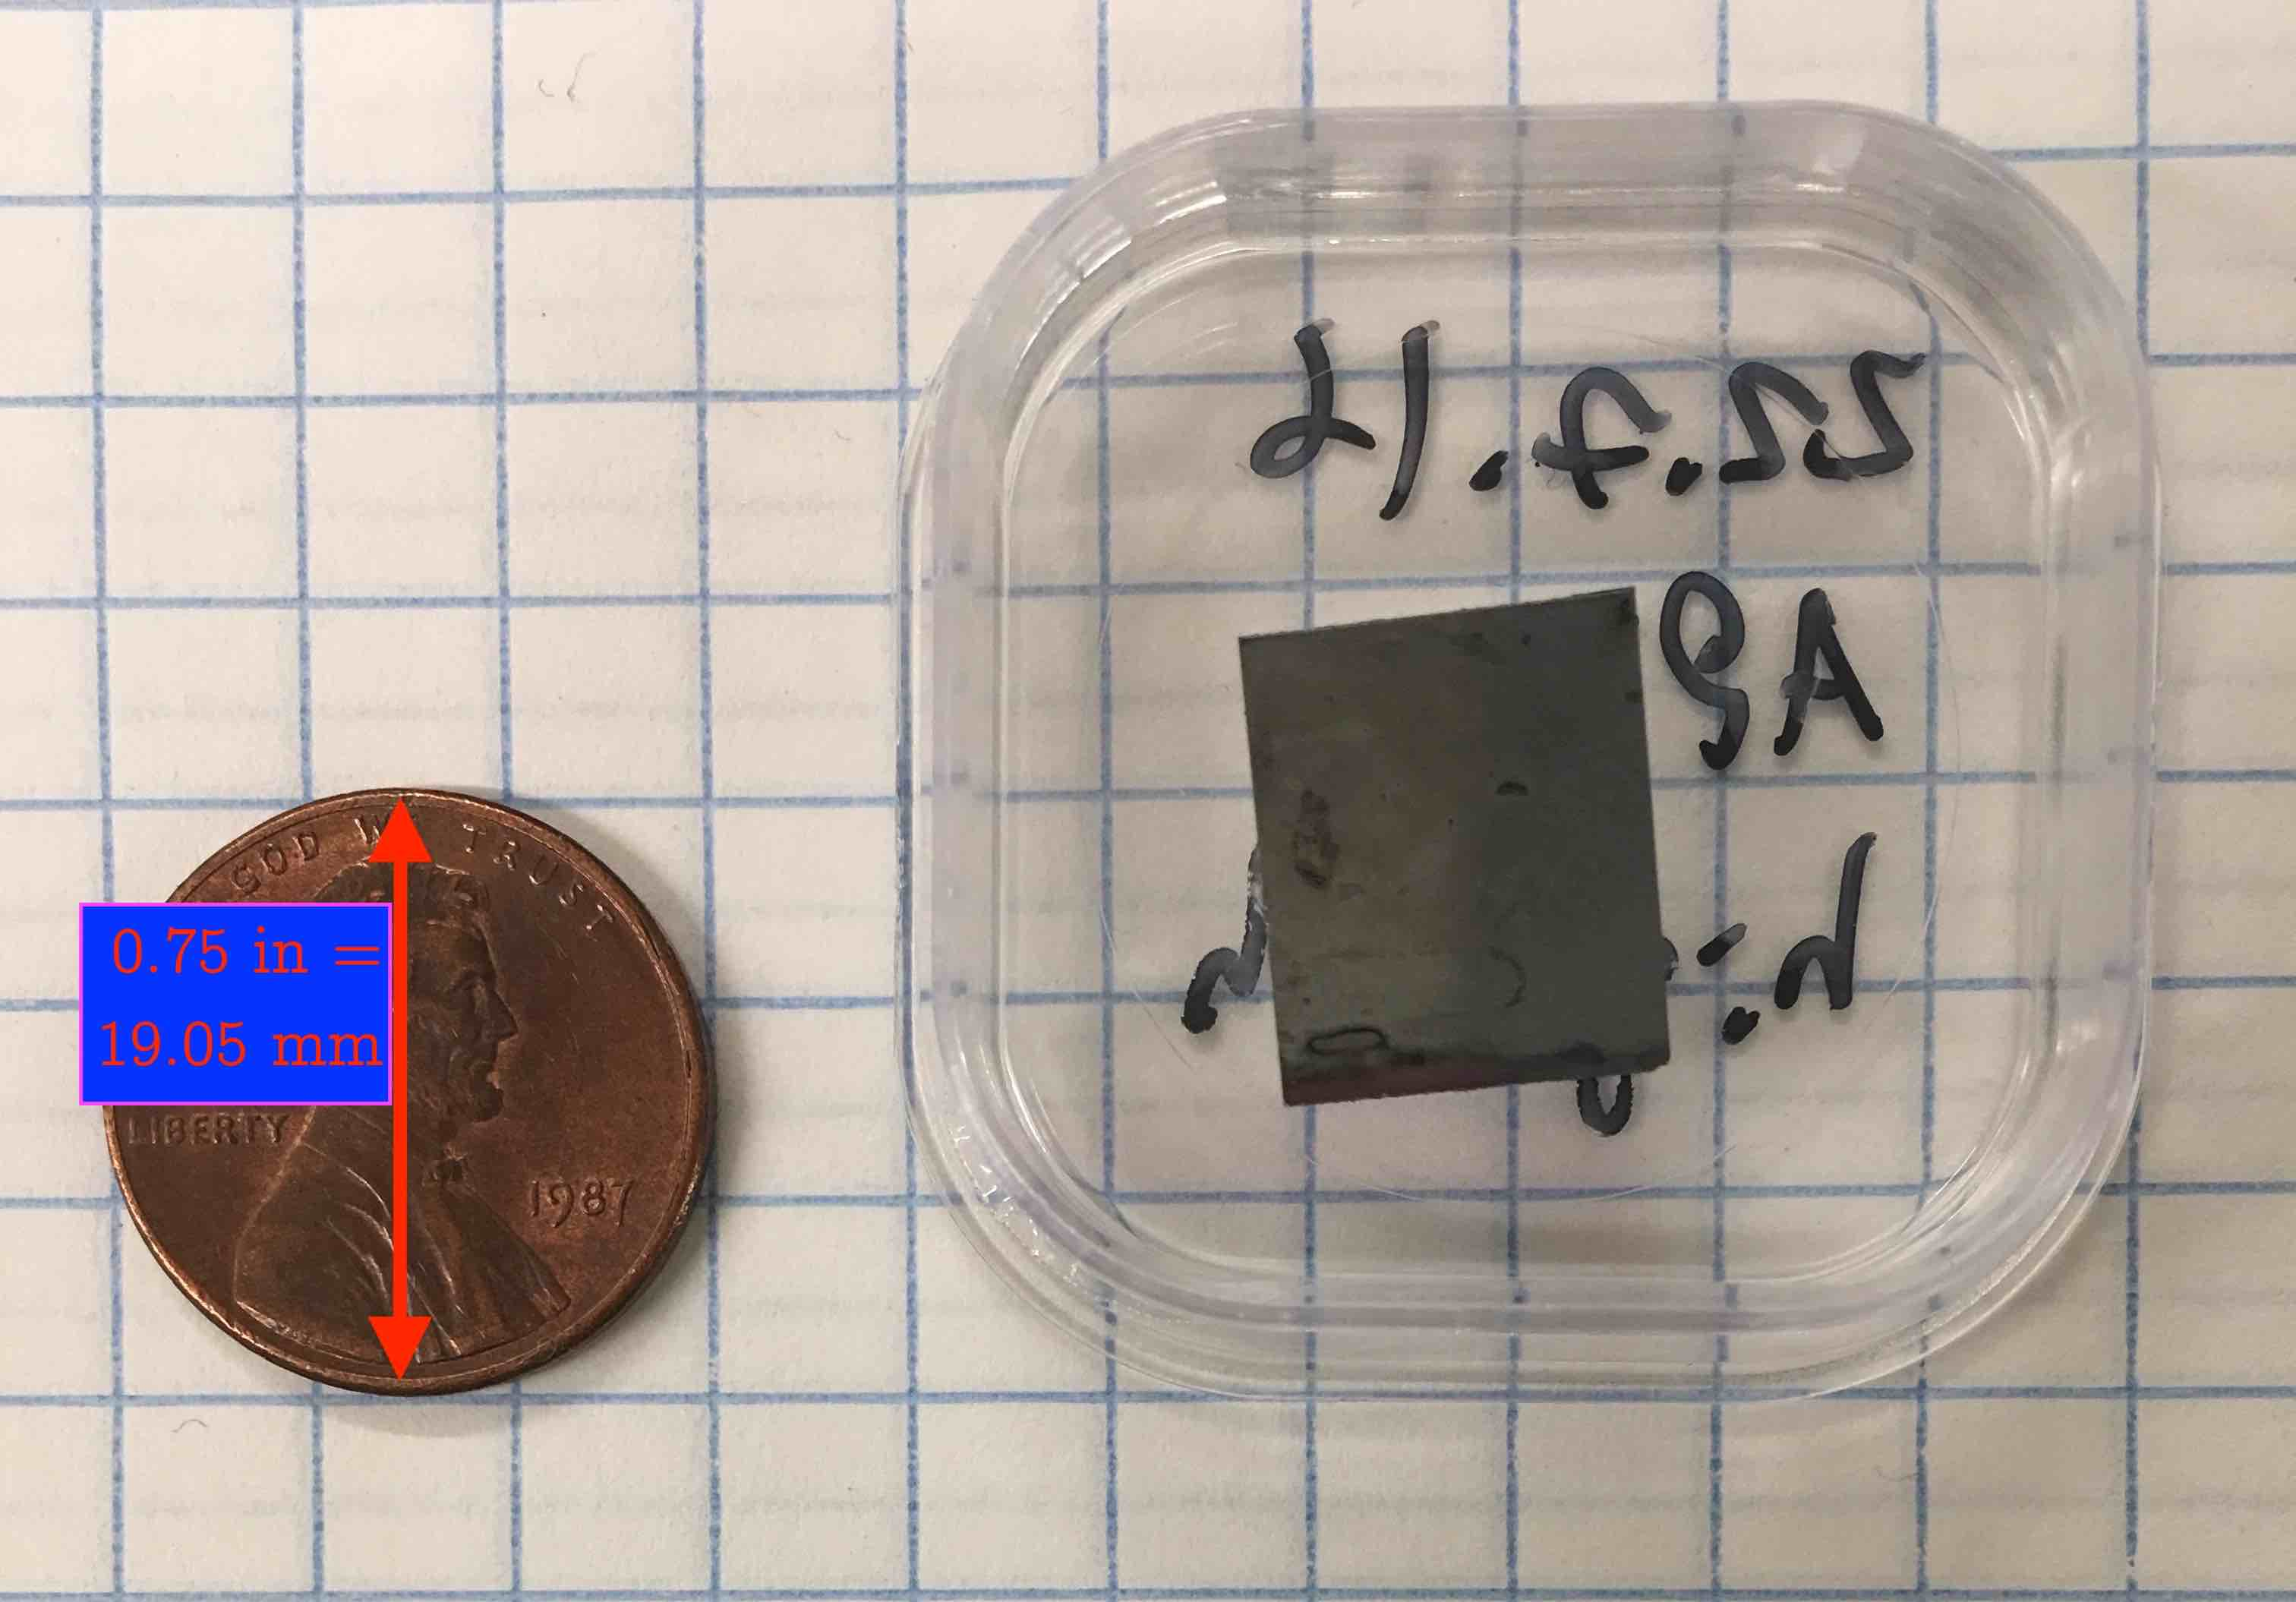
\includegraphics[width=3in]{./images/photo_of_thin_film_sample.jpg}%
%}{%
%  \caption{Top-down photo of the thin film sample of PbS(Th) analyzed in this work. US penny included for scale.\label{photo_of_thin_film_sample}}%
%}
%\capbtabbox{%
%\begin{tabular}{|l|l|}\hline
%Substrate						&	GaAs (100) \\\hline
%Dimensions					&	1 cm x 1.5 cm \\\hline
%Film thickness					&	$\sim$500 nm \\\hline
%Grain size						&	$\sim$150 nm \\\hline
%Th 228 concentration			&	0.15 ppm \\\hline
%Total activity*					&	65 Bq \\\hline
%Sample creation date			&	22 Jul 2016\\\hline
%\end{tabular}
%}{%
%  \caption{Sample properties reported by Templeman et al. 2017 \cite{Templeman2017}. * Total activity measured a brief but unknown time after sample preparation. \label{sample_properties}}%
%}
%\end{floatrow}
%\end{figure}
\section{Transient grating spectroscopy}
838 days elapsed between sample preparation and TGS measurements, which was presumed to be plenty of time for radiation damage to accumulate to a maximum in the sample. After initial calibration runs with tungsten, two sets of runs were conducted with one annealing stage between them. Before annealing, five runs where conducted with the vacuum chamber at <12 mTorr and no temperature control (i.e. roughly room temperature). The annealing was conducted at 280 $^\circ$C and $\sim$15 mTorr for 3 hours. The sample was allowed to cool naturally until it hit 90 $^\circ$C, at which point the chamber was exposed to atmospheric pressure (700 mTorr) to assist cooling. At 30 $^\circ$C, pumping was resumed to evacuate the chamber once again. When the pressure descended below 25 mTorr, 90 post-annealing runs were conducted at 2 minute intervals. The DAQ faulted after 3:02 hrs, so an additional five runs were conducted at 2 minute intervals at about 8mTorr.

\section{TGS Data Analysis}
The mathematical foundation of TGS data analysis is discussed in depth in two papers by Dennett \& Short \cite{Dennett2017, Dennett2018}. These methods were in turn implemented in a library of MATLAB functions in Dennett and Short 2018 and hosted on GitHub \cite{dennett_short_github}. The functions of this library were utilized in ew MATLAB scripts written for this work. All scripts and functions used in this work are publicly available online in a GitHub repository \cite{Sergheyev2019}. Any modifications of the original library from Dennett and Short 2018 can also be found there.

\section{Radiation damage}
\subsection{Decay chain}
The decay chain of thorium 228 was computed with the Universal Decay Calculator, available online \cite{wise_calculator}. Thorium 228 was assumed pure at creation, then aged 913 days ($\approx$2.5 years) before being added, along with its decay products, to the chemical bath solution to grow the PbS thin film. It is assumed that thorium 228 and all of its daughters were incorporated in the to PbS crystal lattice in proportion to the concentrations with which they were present in the chemical bath. For instance, if the ratio of radium 224 to thorium 228 were 2:1 in the chemical bath, then we expect that ratio to hold in the solid solution of the thin film as well. It is not currently known how accurate this assumption is, or if epitaxial growth shows a preference for some daughters on a chemical basis over others.

After the thin film was prepared, its total activity was measured to be 65 Bq, which we can use to extrapolate the activity at the time of the TGS measurements. If we assume this activity of 65 Bq represents the complete inventory of radionuclides in the thin film at $t = 913$ days (i.e. neglecting how different emissions are attenuated differently and detected with different efficiencies), then we can work backward to determine what initial activity of Th-228 must have been on the day it was prepared.

Take as an ansatz that the initial activity of Th-228 was 1.0 Bq when pure at $t=0$. Age it 913 days, and we get a decay chain inventory with total activity 2.843 Bq. Thus, an activity of 22.86 Bq must have been initially present to result in a total activity of 65 Bq at $t=913$. This method was used to compute the inventory at different times, as shown in Table \ref{ansatz_decay_chain_inventory}. The final time, $t=1751$, is the time at which the experiment in this work took place (i.e. TGS and annealing).

\begin{figure}[th]
\begin{center}
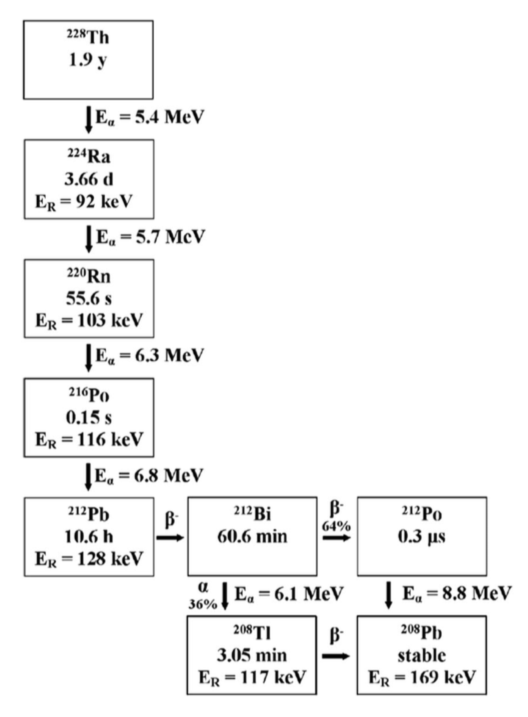
\includegraphics[width=.5\textwidth]{./images/Th_228_decay_chain.png}
\caption{The decay chain of thorium 228 is a subset of the decay chain of the more familiar isotope thorium 232. Shown are the daughters, alpha energies, and daughter recoil energies. Where nuclides are known to emit alphas of more than one energy, the energy shown is an average of all alpha energies weighted by their intensity (i.e. percent of decays)\cite{Templeman2017, CRC}.}
\label{Th_228_decay_chain}
\end{center}
\end{figure}

\begin{figure}[thb]
\begin{center}
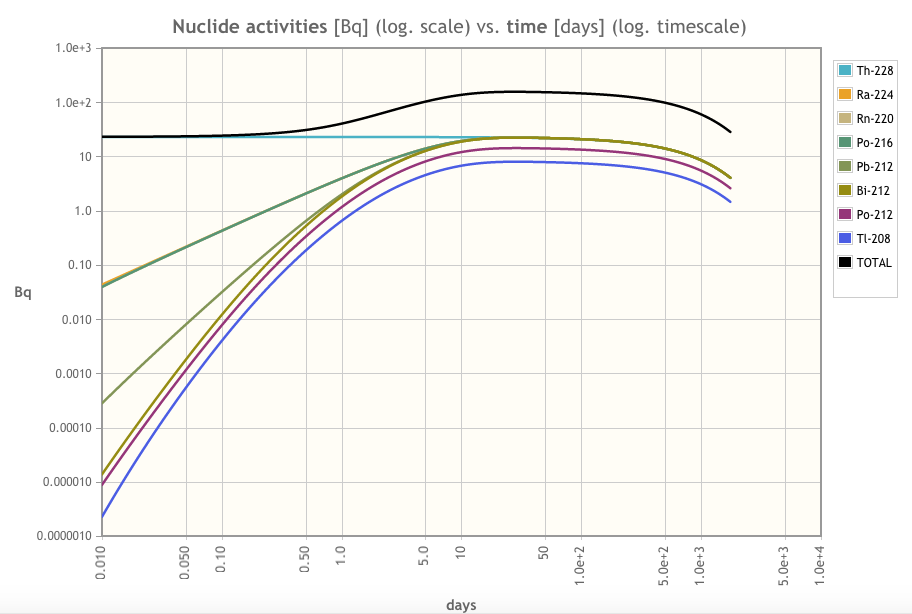
\includegraphics[width=\textwidth]{./images/thorium_decay_chain_plot.png}
\caption{Plot of the time evolution of the Th-228 decay chain inventory, with each species' activity also plotted. $t=0$ is the time of Th-228 preparation. Th-228 activity decreases monotonically, but total activity increases before falling off. Total and all individual activities are declined by the time of sample preparation. All non-stable daughters have shorter half-lives than Th-228, but secular equilibrium with Th-228 is never attained because Pb-212 is more stable than its parent Po-216.}
\label{plot_of_inventory_time_evolution}
\end{center}
\end{figure}


\begin{table}[th]
\begin{center}
\begin{tabular}{|r|c|c|c|}\hline
		&	$t=0$	&	$t=913$	&	$t=1751$	\\\hline
Th-228	&	22.86	&	9.241	&	4.024	\\
Ra-224	&	0		&	9.290	&	4.045	\\
Rn-220	&	0		&	9.290	&	4.045	\\
Po-216	&	0		&	9.290	&	4.045	\\
Pb-212	&	0		&	9.296	&	4.048	\\
Bi-212	&	0		&	9.297	&	4.048	\\
Po-212	&	0		&	5.956	&	2.594	\\
Tl-208	&	0		&	3.340	&	1.454	\\\hline
Total		&	22.86	&	65.00	&	28.30	\\\hline
\end{tabular}
\end{center}
\caption{Computed inventory of complete thorium 228 decay chain at different times: (a) at time of Th-228 preparation; (b) at time of CBD of PbS(Th) thin film; (c) at the time of radiation damage study with TGS. All times given in days and all activities given in Bq \label{ansatz_decay_chain_inventory}}
\end{table}%


\subsection{SRIM/TRIM}
SRIM 2013 \cite{srim_website} was utilized to simulate alpha and recoiling daughter transport in the lead sulfide thin film in order to get an estimate of the damage caused by the decay chain presented above. SRIM, an abbreviation of Stopping and Range of Ions in Matter, is a closed-source suite of programs to perform a number of calculations and simulations related to user specified ions incident upon a user defined material target. In one program, SR, ion range in a target is calculated directly with tabulated values, interpolation, and heuristics. TRIM, which is an abbreviation of Transport of Ions in Matter, uses a monte carlo simulation of probabilistic ion collisions in the material to construct cascades, and thus report on basic damage formation.

SR and TRIM were used first to estimate the range of both alphas and recoiling daughters within PbS(Th), and secondly to estimate the damage rate in DPA/s of the radiation emitted by the thorium decay chain. Input files can be found in the GitHub repository for this work \cite{Sergheyev2019}, but important values used across the SRIM suite are summarized in Table \ref{trim_inputs}.

\begin{table}[thb]
\begin{center}
\begin{tabular}{|r|r|}\hline
Incident alpha energy	&	5423 $keV$\\
Random seed			&	716381\\
Density				&	7.60 $g/cm^3$ \cite{CRC}\\
\# of particles simulated	&	9999\\\hline
\end{tabular}
\begin{tabular}{|r|r|r|r|}\hline
					&	$^{207}$Pb	&	$^{32}$S		&	$^{228}$Th\\\hline
Stoichiometry (ppb)		&	499999925	&	499999925	&	150		\\\hline
Displacement energy (eV)&	16.4			&	16.4			&	16.4 		\\\hline
Lattice binding energy (eV)&	2			&	2			&	2 		\\\hline
Surface binding energy (eV)&	2.2			&	5.63			&	2 		\\\hline
\end{tabular}
\end{center}
\caption{SRIM/TRIM inputs for calculating range of alpha particles in PbS(Th). 5423 keV is the primary alpha from Th-228 decay \cite{NNDC}. The lattice binding energy and surface binding energy are values recommended by SRIM's creators; as is the unusual and unusually specific choice of random seed \cite{srim_textbook}. 16.4 eV represents half of PbS's crystal binding energy \cite{Tanaka1979}.\label{trim_inputs}}
\end{table}%

According to SR, 5.423 MeV alpha particles incident upon an infinite volume of PbS with 15 ppm Th doping ought to have a range of 18.41 $\mu m$ with a straggling of 1.06 $\mu m$. In TRIM, 9999 alphas were simulated in an infinite medium, which resulted in a similar range of 18.4 $\mu m$ with a straggling of 0.7488 $\mu m$. Lateral range was under 2 $\mu m$ in both cases, and therefore negligible. In other words, the alpha particles exhibit typical behavior of traveling in a straight line and coming to an abrupt stop. The significance of the range of the alphas compared to the thickness will be discussed later.

Next, TRIM was used to estimate the damage from alphas. In the infinite volume case, TRIM reports 366 displacements/alpha, 23 of which result in recombination of an interstitial and a vacancy. When the layer thickness was reduced to 500 nm to match the thin film, the displacements/alpha dropped to 2.


% Repo for code: http://dx.doi.org/10.5281/zenodo.1239854 
%
%
% Atmospheric pressure is 760 Torr
% run_notes.txt:
%BGU Experiment
%Sample: "22.7.16 high Th"
%Date: 2018/11/07
%
%- Pre anneal measurements at <12mTorr
%- During the anneal
%- 11:32 30mTorr (right as it hit 280C)
%- 11:35 14mTorr
%- 11:45 10mTorr
%- 12:00 9mTorr
%- 14:31 8mTorr, heater turned off
%- 15:00 crack to air on cool down at 90C
%- 15:09 start to pump again at 30C
%- 15:15 start 4 hour post-anneal @ 25mTorr
%- 15:30 10mTorr
%- bottomed out at 8mTorr again for room temp ost anneal
%
%- Set was four hour post anneal and cool at 5000 traces per batch on 2 minute intervals
%- DAQ faulted after 3 hours and 2 minutes on post_anneal_00
%- Do a series of 5x5000 starting at 19:10ish
%- stop measurement after those 5. 
%- final temperature record saved in "temp_rec_04.csv" for the entire experiment.
%
%
%

